% \documentclass{WHUBachelor}% 选项 forprint: 交付打印时添加, 避免彩色链接字迹打印偏淡. 即使用下一行:
 \documentclass[forprint]{WHUBachelor}
  \lstset{ 
    basicstyle=\small,% 
    escapeinside=``,% 
    keywordstyle=\color{red} \bfseries,% \underbar,% 
    identifierstyle={},% 
    commentstyle=\color{blue},% 
    stringstyle=\ttfamily,% 
    %labelstyle=\tiny,% 
    breaklines=true,
    extendedchars=false,% 
    linewidth=\textwidth,% 
    numbers=left,% 
    numberstyle=\tiny \color{blue},% 
    frame=trbl% 
    }


\begin{document}
%%%%%%% 下面的内容, 据实填空.

\title{实验项目二:用户程序加载器的实现}
\Cschoolname{数据科学与计算机学院}          % 学院名
\Cmajor{计算机科学与技术}                  % 专业中文名
\StudentNumber{16337237} % 填写自己的学号
\author{王永锋}                            % 作者名字
\Csupervisor{凌应标}        %指导教师中文名、职称
\date{二〇一八年三月九日}                    % 日期, 要注意和英文日期一致!!

%----------------------------------------------------------------------------
\pdfbookmark[0]{封面}{title}         % 封面页加到 pdf 书签
\maketitle
\frontmatter
\pagenumbering{Roman}              % 正文之前的页码用大写罗马字母编号.
%-----------------------------------------------------------------------------
% \include{includefile/frontmatter}    % 加入摘要, 申明.
%==========================把目录加入到书签==============================%%%%%%
\pdfbookmark[0]{目录}{toc}
\tableofcontents
\mainmatter %% 以下是正文

%%%%%%%%%%%%%%%%%%%%%%%%%%%%%%%%%%%%%%%%%%%%%%%%%%%%%%%%%%%%%%%%%%%%%%%%%%%%%%%%%%%%%
%【实验方案】包括:硬件或虚拟机配置方法、软件工具与作用、方案的思想、相关原理、程序流程、算法和数据结构、程序关键模块,结合代码与程序中的位置位置进行解释。不得抄袭,否则按作弊处理。
%【实验过程】包括:主要工具安装使用过程及截图结果、程序过程中的操作步骤、测试数据、输入及输出说明、遇到的问题及解决情况、关键功能或操作的截图结果。不得抄袭,否则按作弊处理。
%【实验总结】每人必需写一段,文字不少于500字,可以写心得体会、问题讨论与思考、新的设想、感言总结或提出建议等等。不得抄袭,否则按作弊处理。
%【参考文献】(如有要列出,包括网上资源)
%%%%%%%%%%%%%%%%%%%%%%%%%%%--------main matter-------%%%%%%%%%%%%%%%%%%%%%%%%%%%%%%%%%%%%
\chapter{实验目的及要求}

\section{实验目的}

\begin{enumerate}
  \item 理解单道批处理操作系统的原理及实现。
  \item 了解及掌握系统内核加载用户程序的原理。
  \item 学会使用bios中断。
  \item 了解并掌握BIOS中断,能够自己通过修改中断向量表实现新的中断。
  \item 实现一个用户程序加载器。
\end{enumerate}

\section{实验要求}

本次实验,要求需要完成以下目标:\\

\begin{itemize}
  \item \textbf{实现用户程序加载器} \\
  修改参考原型代码,允许键盘输入,用于指定运行这四个有输出的用户可执行程序之一,要确保系统执行代码不超过512字节,以便放在引导扇区。
  \item \textbf{自定义用户程序} \\
  设计四个有输出的用户可执行程序,分别在屏幕1/4区域动态输出字符,如将用字符‘A’从屏幕左边某行位置45度角下斜射出,保持一个可观察的适当速度直线运动,碰到屏幕相应1/4区域的边后产生反射,改变方向运动,如此类推,不断运动;在此基础上,增加你的个性扩展,如同时控制两个运动的轨迹,或炫酷动态变色,个性画面,如此等等,自由不限。还要在屏幕某个区域特别的方式显示你的学号姓名等个人信息。
\end{itemize}

\chapter{实验方案}

\section{实验工具和环境}

本次实验平台\footnote{部分参考\cite{于渊2009orange}}搭建在win10系统的linux子系统上,通过编写shell脚本,连接nasm编译工具,dd二进制文件覆写工具,与bochs虚拟机加载配置文件与镜像(具体工具链详见下\autoref{tab:tools}),实现了\textbf{编写代码后一键启动虚拟机查看结果}。同时,使用bochs虚拟机中提供的bochsdbg.exe工具,还能够对产生的镜像文件进行\textbf{单步调试},不仅大大提高了编写汇编文件后查看实现效果的速度,在命令行中通过发送指令对虚拟机的运行进行单步调试,查看各寄存器和内存,能够迅速定位操作系统中存在的问题并且解决它,从而提高我们的开发效率。考虑到bochs虚拟机由于是软件模拟硬件,速度不仅不稳定而且比较慢,因此后来我采用qemu虚拟机进行查看引导程序的结果。

环境与实验一类似,由于编译方式的变化(实验一只需要编译一个文件,而本次实验二需要编译多个文件,然后将生成的多个二进制文件写入同一个磁盘中),此次运行的脚本\autoref{code:my_shell}也做了相应的修改。同时为了方便,我还在脚本中加入了一个参数,以方便对工具的选择,如“q”则为使用qemu虚拟机运行,“b”则为使用bochs运行,“d”则使用bochsdbg进行单步调试。

同时,比起实验一而言,查看磁盘二进制代码的工具从winhex转变成了hexdump,使用此工具的原因有两个,一个是该工具会忽略字节全为0的行,只输出有数据的磁盘内容,这样我就能够很方便的定位到我自己写入的扇区。另一个原因是该工具在命令行下运行,那样我在进行开发的时候就不用总是切换桌面,一个vscode加上内置的命令行中断就能够让我完成全部的开发工作。

\begin{table}[htp]
  \caption{本实验所使用的工具链}
  \centering
  \begin{tabular}{cc}
    \toprule
    软件名称 & 用途  \\
    \midrule
    bash & 一个命令行终端,可提供linux的一些命令与执行shell脚本 \\
    nasm & 将x86汇编文件编译成.bin二进制文件 \\
    dd & 将二进制文件的内容写进软盘镜像中  \\
    hexdump & 以十六进制形式查看软盘镜像文件 \\
    bochs & 虚拟机,用于加载装有自定义引导程序的软盘,使用软件模拟,速度不稳定  \\
    bochsdbg & 调试工具,用于给装有自定义引导程序的软盘文件进行调试 \\
    qemu & 虚拟机,用于加载装有自定义程序的软盘,使用硬件模拟,速度稳定且较快 \\
    \bottomrule
  \end{tabular}
  \label{tab:tools}
\end{table}

\subsection{此步骤曾经遇到的问题}

\begin{itemize}
  \item \textbf{没有先清空软盘再写软盘} \\

  在一开始进行开发的时候,原本产生镜像总是特别顺利,修改了二进制文件的的加载区域之后总是能够正常运行,一开始没有留意,直到我发现我做的一些修改并没有在镜像的运行中体现出来。当我发现问题之后,先是使用bochsdbg调试代码,很惊讶的发现我以前的代码仍然保留在镜像中,没有头绪。后来我使用hexdump查看镜像的二进制文件,才看到一些我明明没有写入的扇区居然会有数据!仔细一想吧,才猜到那可能是我以前写入的数据,没有被清除掉。后来在脚本里面加上了这样一条语句实现清空磁盘后,才发现了自己代码的众多bug。
  \begin{lstlisting}
    dd if=/dev/zero of=a.img ibs=512 count=100 conv=notrunc
  \end{lstlisting}
  \item \textbf{在编译错误后仍然运行虚拟机} \\

  一开始的脚本文件写的并不是特别好,即使在编译出现错误之后还运行虚拟机,这样子我每一次运行脚本还要先去看一看有没有出现编译错误。后来了解到nasm编译错误之后会返回0,据此,在原来的编译语句后面加上逻辑控制符“||”,若返回0,则还需要运行后面的语句才能决定整体的返回值,则会退出脚本文件。若正常运行返回1,则不需要运行后面的语句,就能够继续执行下面的语句。
  \begin{lstlisting}
    nasm.exe -f bin my_mbr.asm -l my_mbr.list -o my_mbr.bin    || { echo "nasm complied failed"; exit 1; }
  \end{lstlisting}
\end{itemize}

\section{程序功能说明及大致思路阐述}

这里会对程序的大致运行流程进行一个粗略的描述,同时罗列了当前系统内核支持的功能。

\subsection{程序大致思路阐述}

\begin{enumerate}
  \item 一开机,处于软盘第一个扇区的引导程序加载第2-12个扇区,作为系统内核,并将控制权转交给系统内核。
  \item 系统内核刚开始运行,需要先对各段寄存器进行重定位,并安装8号和40号中断,安装完之后,输出相应信息,提醒用户按“enter”继续运行,以进入系统内核主菜单。
  \item 调用一个过程打印系统内核主菜单,并将程序控制权停留在主菜单中的键盘读取循环中,不断查询键盘缓冲区,一旦有按键,马上判断是否需要加载用户程序及加载哪一个用户程序。如果有对应选项,则将对应的用户程序从磁盘中加载到内存地址为0x1000:0x0000的区域,并将控制权转交给用户程序执行。
  \item 用户程序\footnote{格式与.com类似,差别在于地址从0x10000开始而不是从0x0100开始}正常执行,执行结束后,用户显式调用 "int 40h"\footnote{类似于dos操作系统下功能号为4ch的“int 21h”}实现返回到操作系统内核。
  \item 通过修改“int 8h”定时器中断,实现边框旋转,修改该中断的主要原因是想尝试使用该中断实现分时系统,现在先学会如何使用定时去中断。
\end{enumerate}

\subsection{程序功能说明}
本程序(完整程序代码见附件)实现了以下功能(主界面可见\autoref{fig:main_screen2})。
\begin{enumerate}
  \item \textbf{按下1。}执行第一个用户程序,该用户程序为一个单独的会弹跳的笑脸\footnote{ASCII代码为02h},范围限制在左上角1/4的区域。
  \item \textbf{按下2,3,4。}执行第2,3,4个用户程序,与1类似,不过范围分别限制在了右上角,左下角,右下角区域。
  \item \textbf{按下l。}运行我在以前的实验一实现的程序,做的修改不多,主要是起始地址从7c00h改成了0x10000。在此用户程序中,按下c可清屏,按下d可以展示我自己的名字。
  \item \textbf{按下t。}运行我的一个测试程序,仅仅输出两句话。
  \item \textbf{在用户程序中:按q。} 在任何一个用户程序中,只需要按q,就可以返回到系统内核主菜单。
\end{enumerate}

\section{代码实现1-"my\_mbr.asm"}
此份代码参考了老师的代码并且做了一些修改。

\begin{enumerate}
  \item 保留了显示字符串的过程(实际上由于运行时间过快,看不到该串字符串的实现,直接转到了内核中)。
  \item 读取软盘的扇区,修改成了从第二个扇区开始,加载10个扇区到内存地址为0x0100:0x0000的地方。\footnote{本系统内核固定在内存地址为0x0100:0x0000处开始。}
  \item 通过jmp指令,跳转到系统内核的第一条指令。
  \begin{lstlisting}[language={[x86masm]Assembler}]
    jmp my_core_header_address ;该常量为0x1000
  \end{lstlisting}
\end{enumerate}

\section{代码实现2-"my\_core.asm"}
此份代码中,除了8号中断的安装和执行\footnote{参考自一个汇编语言实现射击游戏中的代码\cite{hit_plane}},以及读取扇区过程\cite{read_sector},其他的代码都是自己写的。 

代码分为四个段:内核首部,内核代码段,内核数据段,内核栈段\footnote{如此分段参考自《x86汇编:从实模式到保护模式》\cite{2013x86汇编语言从实模式到保护模式}}。为了方便说明代码各部分作用,将代码段拆分为公用例程段,自定义中断,及内核入口三部分分别说明。同时数据段与栈段共同说明。

\subsection{内核首部}
主引导程序跳转到内核之后,运行的第一条指令就在首部的redirect过程中。先暂时将数据段指针设置为内核首部以方便对内核首部的段表的修改,然后就对段表中各个段的地址进行重定位。\footnote{重定位是指,原本段表存有的数据仅仅是相应段在代码中的汇编地址,是相对偏移地址,而不是真实的物理地址。通过将该偏移地址逻辑右移四位,然后加上此时程序实际所在内存地址的段地址(0x1000),便得到代码段,数据段,栈段在运行期间的真实段地址。}最后通过jmp far指令,读取代码段地址和第一条指令的偏移量,修改cs和ip,转到内核入口开始执行。
\begin{lstlisting}[language={[x86masm]Assembler}]
section my_core_header vstart=0
; 重定向段表
redirect:
    ; 将ds指向内核首部,为之后重定位内核段表
    mov ax, 0x0100
    mov ds, ax
    ; 重定位内核段表
    shr word [code_segment], 4
    add word [code_segment], 0x0100
    shr word [data_segment], 4
    add word [data_segment], 0x0100
    shr word [stack_segment], 4
    add word [stack_segment], 0x0100
    jmp far [code_entry]
; 内核首部,指明第一条指令偏移地址,及代码段段地址
; 经过上面的重定向程序后,能够将下面的汇编地址转变成实际运行的地址。
code_entry dw code_start
code_segment dw section.code.start
data_segment dw section.data.start
stack_segment dw section.stack.start
core_entry dw core_start
\end{lstlisting}

\subsection{内核代码段-公用例程段}
该部分的代码主要是一些函数,一般在代码段中的内核入口使用call调用来简化内核的结构。该部分的代码行数比较多,同时技术含量不高,就不把代码放在报告中。其中ReadSector过程参考了网上的一篇博客\cite{read_sector}。

\begin{table}[htp]
  \caption{内核代码段-公用例程段中的各过程作用说明}
  \centering
  \rowcolors{1}{White}{Lavender}
  \begin{tabular}{lp{11cm}}
    \toprule
    过程名称 & 过程说明 \\
    \midrule
    clean\_screen & 该过程用于清屏。 \\
    display\_core\_massage & 该过程用于显示内核的加载信息,屏幕输出一段字符串表明系统内核加载完成,该过程运行与内核态。 \\
    show\_welcome\_screen & 该过程用于打印系统内核菜单,该过程运行于内核态,意味着该过程依赖内核中段寄存器的正确取值。 \\
    ReadSector & 该过程能够将扇区号(从0开始递增的序列),翻译成相应的柱面号,起始扇区,磁头号,并且读取对应数量的扇区。 \\
    load\_com\_user\_program & 传入参数,放在ax中,表明需要从该扇区号开始读取18个扇区,并在内部设置为读进0x1000:0x0000,然后调用ReadSector过程翻译扇区号并加载对应扇区。 \\
    get\_random & 该过程可以获取0-7范围的随机数,并写回到al中,同时加上114(为了使al翻译成白背景色随机字体色)。     \\
    \bottomrule
    \hiderowcolors
  \end{tabular}
  \label{tab:code-segment-common}
\end{table}

\subsection{内核代码段-自定义中断}
该部分的代码分两种,一种是安装中断,另一种是实际的我自定义的中断例程。这里以int40h举例,说明我的代码的实现方式。完整代码课件\autoref{code:int40h}

\begin{table}[htp]
  \caption{内核代码段中自定义中断部分过程的说明}
  \centering
  \rowcolors{1}{White}{Lavender}
  \begin{tabular}{lp{11cm}}
    \toprule
    过程名称 & 过程作用 \\
    \midrule
    install\_int40 &  该过程用于修改中断向量表,从而使得0x40号中断指向我自己编写的中断程序。 \\
    int40\_for\_return & 执行该中断,就能够从用户程序中返回到系统内核,并且将段寄存器设置为内核态。\\
    install\_int8 & 该过程用于修改中断向量表,从而使得0x08号中断指向我自己编写的中断程序。 \\
    new\_int8 & 执行一次该中断,屏幕边缘的所有符号就逆时钟转动一格。  \\
    \bottomrule
  \hiderowcolors
  \end{tabular}
  \label{tab:code-segment-ivt}
\end{table}

\subsubsection{int 40h 的安装}

int 40h 的安装,直接修改对应的中断向量表项即可。\\
  \begin{lstlisting}[language={[x86masm]Assembler}]
    ; 安装 int 40 主要代码
    mov ax, 0
    mov ds, ax
    mov ax, cs
    mov word [0x40*4], int40_for_return 
    mov word [0x40*4+2], ax
  \end{lstlisting}
\subsubsection{int 40h 的执行}  
int 40h 的实现的机制与中断的原理息息相关。\\
  在用户调用中断的时候,机器会先将标志寄存器,cs, ip依次push进用户栈中。为了保证用户栈不会改变\footnote{若不pop出来,切回到内核后,用户栈将会多出三项,导致用户栈发生改变。},先将用户栈中的三项依次pop出来,然后push标志寄存器,内核地址和指令偏移量,iret就可以直接读取被我修改后的地址,返回到内核中。 \\
  这里有一个很重要的问题,在后面push新地址的时候,我们不能够再push到用户栈了,因此,在push新地址前,先将各段寄存器切换到内核中的段寄存器\footnote{这里做的工作与初始化内核类似,同时各段地址从内核首部的段表取得。}(除了cs),保证段寄存器已经是内核状态后,将新地址push到内核栈后,此时的iret就会将内核栈中的新地址pop出来,将cs,ip修改为正确的值,进而将控制权转交给内核的功能入口。从而实现用户程序转入内核的蜕变。
  \begin{lstlisting}[language={[x86masm]Assembler}]
    ; 在用户栈中
    pop ax ; pop 原调用中断的偏移地址
    pop ax ; pop 原调用中断的段地址
    pop bx ; pop 用户的标志寄存器

    ; 修改段寄存器:ds, ss, es
    mov ax, core_header_data_segment
    mov ds, ax
    mov es, ax
    mov ax, word [core_stack_segment_header_offset]
    mov ss, ax
    mov sp, core_stack_length

    ; 保证栈为内核状态
    push bx ; push 标志寄存器 可能要修改
    push word [core_code_segment_header_offset]
    push word [core_entry_header_offset]

    ; 设置数据段寄存器
    mov ax, [core_data_segment_header_offset]
    mov ds, ax

    iret ; 成功回到内核
  \end{lstlisting}

\subsection{内核代码段-内核入口及程序返回点}

该部分的代码可分为内核初始化以及内核功能入口(即内核返回点)。这里的代码可见\autoref{code:my_core_entry}\\
\begin{enumerate}
  \item \textbf{内核初始化} 先使用重定向后的段表修改段寄存器,然后调用安装中断例程,安装0x40号和0x08号中断,最后打印完内核加载消息后转到读取键盘的循环中,一旦键入“enter”,则进入系统内核主菜单。
  \item \textbf{内核功能入口(内核返回点)} 先清屏,打印主菜单,然后就进入读取键盘的循环,根据按键的不同,选择加载不同扇区的内容并执行。当用户程序返回的时候,也是返回到该段代码的第一条指令处。
\end{enumerate}

\subsection{内核数据段及栈段}

这部分就不详细说明了,需要说明的一点是,我为内核创建了一块大小为256字节的栈空间,用于内核中代码的执行。该栈区是内核独有的,用户程序无法访问内核的栈\footnote{由于当前仍然属于16位实模式,这里的无法访问并没有权限来限制,如果显式的将栈的段地址修改为内核的栈的段地址也还是可以访问的,但一般.com中不会修改栈的段地址。}。用户同样无法访问内核的数据。同时,在汇编代码中将数据段和栈段使用以下声明来写出来,能够生成正确的汇编地址,以便之后使用段寄存器正确的读取到响应的数据。 \\

\begin{lstlisting}
  section data align=16 vstart=0
  ;数据段。。。。
  section stack align=16 vstart=0
  ;栈段。。。。。 
  ; vstart=0 表明汇编的时候该段一下的地址为相对于当前段的偏移量,而不是相对于整个程序的偏移量
\end{lstlisting}

\section{代码实现3-"my\_user\_program\_1.asm"}

用户程序1至4的实现是相似的\footnote{仅仅是笑脸弹跳范围不同},因此这里只展示第一个用户程序的代码并做相关说明。

用户程序的效果,就是实现了一个笑脸\footnote{ASCII码为02h}在指定的范围内上下左右跳动,碰壁反弹,虽然是与实验一中老师给的代码实现的功能类似,但是由于那一份代码写得较为冗长,而且还有飞到对角线就会飞出去的bug,因此这一次自己重写了弹跳的代码。同时,与dos中的"int 21h"中断类似,在用户程序中通过显式的调用“int 40h”来返回到系统内核中。
\subsection{弹跳的代码}
弹跳代码经过重写,运行的流程和逻辑发生较大的改变,运行流程图如\autoref{fig:flow}。完整代码可见\autoref{code:jump}。

\begin{figure}[htp]
  \centering
  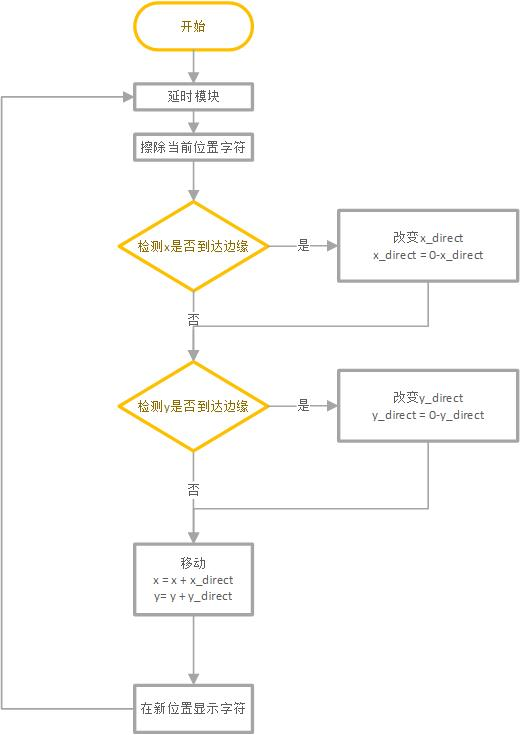
\includegraphics[width=13cm]{"./figure/figure.jpg"}
  \caption{代码运行流程图}
  \label{fig:flow}
\end{figure}

\cleardoublepage

\subsection{显式使用int40h中断返回操作系统}
为了减少该系统内核实现的用户加载器对代码格式的要求。仿照.com文件中使用如下代码来返回dos操作系统的操作(如下列代码)
\begin{lstlisting}
  mov ax, 4c00h
  int 21h
\end{lstlisting}
我在用户程序中,显式的调用自定义的“int 40h”中断例程来做到返回用户的操作系统。
\begin{lstlisting}[language={[x86masm]Assembler}]
check_keyboard:
  mov ah, 01h
  int 16h
  ; 不断查询键盘缓冲区的状况
  ; 若有按键,则zf为0,若无按键,则zf为1,跳回去继续查询
  jz clean_current_char
  ; 有字符输入,从al中读取键盘输入
  mov ah, 00h
  int 16h

  cmp al, 'q' ; 如果键入q则退出用户程序返回操作系统
  jnz check_keyboard
  int 40h
\end{lstlisting}

其实也想过使用“int 9h”来使用键盘产生硬件中断,停止用户程序的执行返回到操作系统中,但是这样的操作与正常用户的需求并不一直。在运行用户程序的时候,用户程序何时终止运行,应该是用户说了算,因为只有用户才知道代码运行到哪里才完成了该用户程序的任务。为了给用户提供主动退出用户程序的方法,也为了与执行真实.com文件的用户体验类似,我采用了自己设置新中断用于返回操作系统内核的方法。

\chapter{实验结果}

\section{系统内核主菜单}

本程序经nasm编译后在qemu虚拟机下运行的效果可见\autoref{fig:main_screen}与\autoref{fig:main_screen2},其中\autoref{fig:main_screen2}中的边框可以逆时钟旋转同时随机地改变颜色。
\begin{figure}[htp]
  \centering
  \begin{minipage}[t]{0.5\linewidth} 
  \centering
  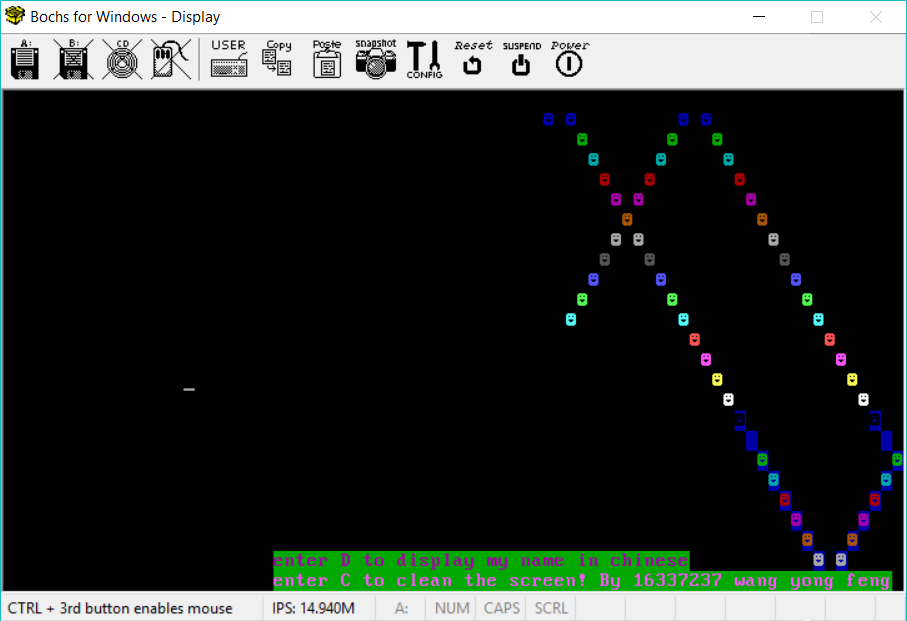
\includegraphics[width=10cm]{"./figure/main_screen.png"}
  \caption{自定义引导程序的主界面}
  \label{fig:main_screen}
  \end{minipage}

  \begin{minipage}[t]{0.5\linewidth} 
  \centering
  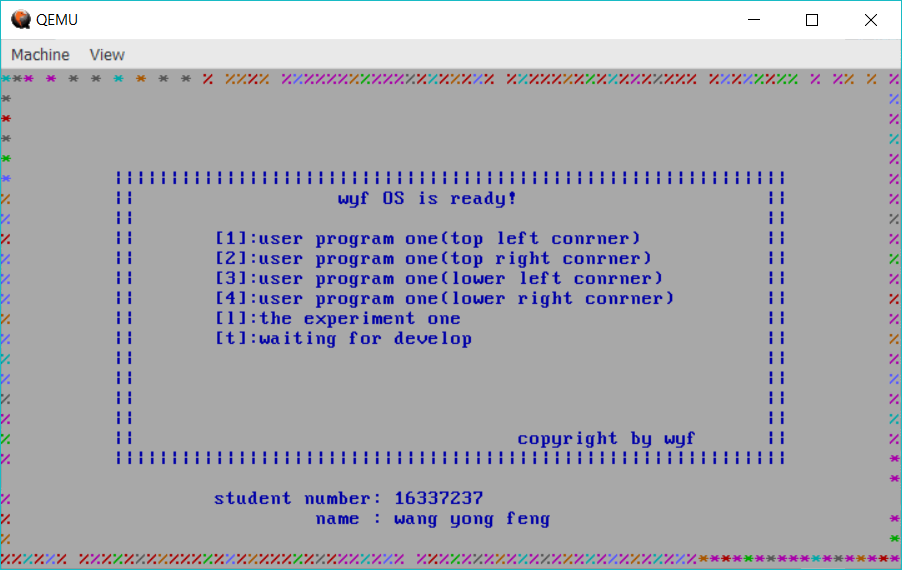
\includegraphics[width=10cm]{"./figure/main_screen2.png"}
  \caption{自定义引导程序按下D后的界面}
  \label{fig:main_screen2}
  \end{minipage}
\end{figure}
\\
\section{执行用户程序并返回到系统内核}
按下1键,进入用户子程序1。用户程序1为笑脸在左上角范围内弹跳,按下q后就能够返回到系统内核主界面。同时,我也将实验一中的程序,加了很少的修改,就能够让我的系统内核加载进内存中顺利执行,同时还能够按q返回。\footnote{具体的修改有修改了起始地址为0x10000,另一个修改是在代码中添加了触发int 40h的按键检测模块。}
\begin{figure}[htp]
  \centering
  \begin{minipage}[t]{0.5\linewidth} 
  \centering
  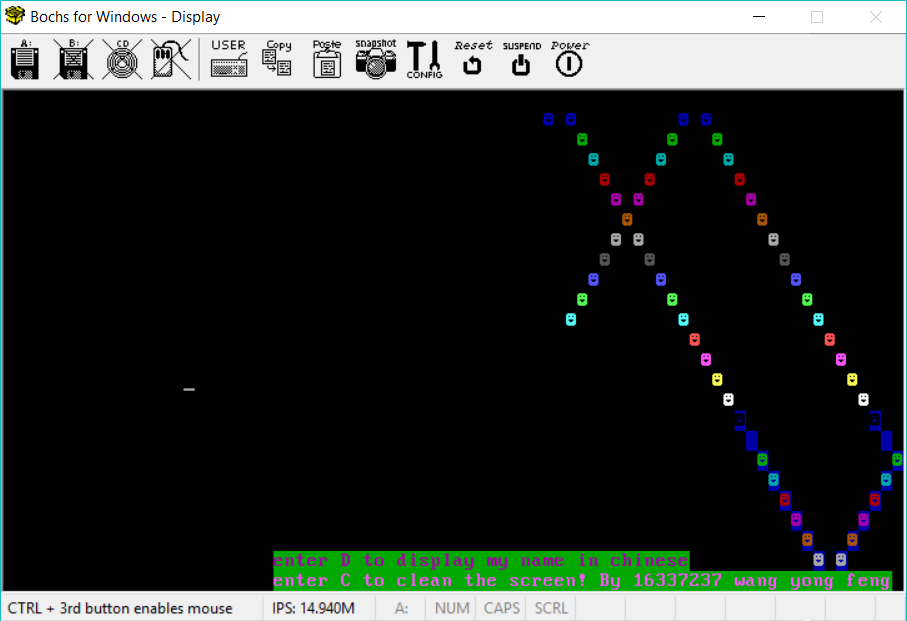
\includegraphics[width=10cm]{"./figure/main_screen.png"}
  \caption{用户程序1的界面}
  \label{fig:main_screen}
  \end{minipage}

  \begin{minipage}[t]{0.5\linewidth} 
  \centering
  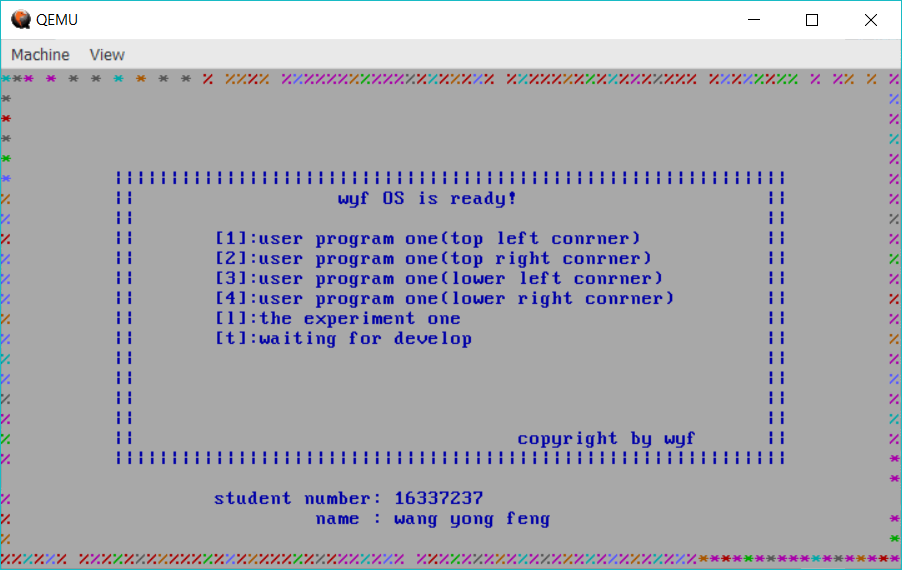
\includegraphics[width=10cm]{"./figure/main_screen2.png"}
  \caption{实验一种的程序的界面}
  \label{fig:main_screen2}
  \end{minipage}
\end{figure}

\chapter{实验总结}
这是实验二的实验总结。

这一次操作系统实验需要实现的是加载器,功能是通过加载器,将处于磁盘中的程序,加载到内存中指定位置,并将处理器的控制权转交给用户程序执行,用户程序执行完毕后,将控制权归还给操作系统内核。

在实现的过程中,其实遇到的问题还蛮多的,一个最大的问题就是关于重定向地址的问题。内核中的段表在汇编完成之后,其实并不是正确的物理地址,里面的地址仅仅是对应的代码相对于第一条代码的汇编地址,可以说是偏移量,但是要处理成正确的段地址,还需要在该地址前加上实际内存的加载地址,并右移四位,才能得到真实的段地址。这里有两个地方需要注意,第一个是各个段的地址要保证低四位为0,这就意味着我需要用align=16这样的语句显示指明对齐方式,第二个问题是在何处进行重定位,我参考过《x86汇编:从实模式到保护模式》那样在调用者处进行重定向,可是由于我有些地方没有处理好,一直重定向失败,如忘记将段地址左移四位等问题,后来索性将重定向的工作放在了调用者处完成(如这内核段表的重定向过程放在了内核首部),这样其实并不正确,下一次实验还是需要改回来的。

严格的来讲,这一次的程序实现的功能仅仅是加载,不足以称之为内核,但它却也有了一点宏内核的雏形。这一次内核代码的组织方式参考了《x86汇编:从实模式到保护模式》中的组织方式,将程序分为首部,代码段(公用例程段+入口段),数据段及栈段,并通过设置段寄存器的方式,将处理器处于内核态的状态与处于用户态的状态明确的区分开来。同时,内核中还有一些只有处于内核态的时候才可以正常执行的过程,这可以类比为宏内核中的系统调用。

但这还不够,用户程序能够调用的与系统调用类似的仅仅是一个自定义的int40h中断,其余啥都没有,这意味着用户程序需要做很多很多的事情来完成自己的工作,并且加载该用户程序的操作系统没能提供为用户程序提供更多的服务,由此看来,这样的操作系统还有很多的工作未完成,我们之后的路还很长。

分时系统,是我所希望实现的一个功能。目前的操作系统,同一个时间只能加载一个程序执行,无法做到同时加载多个程序并发的执行。我也粗略的想过怎么实现,大概就是使用定时器发出中断,将当前正在运行的程序中止并保存现场,然后转入内核由调度器决定下一个运行的程序并执行。为了完成实验二已经花了很长的时间了,也暂时实现不了分时系统,不过为了为以后打下基础,就尝试用了定时器定期发送中断,实现边框的转动。这个定时器中断的代码借鉴自一个使用x86汇编语言时间的射击游戏中的代码,很奇怪的是,相关的资料网上却很少,也找不到一个比较系统的教程,因此到现在,对定时器中断的原理还不是特别清晰。

从用户程序返回到系统内核主菜单,也是一个有点难实现的地方,因为这里涉及到对中断的深刻理解。中断是BIOS对计算机管理员隐藏硬件细节的一个重要的方式,这意味着中断的时候计算机做了一些对程序员不可见的工作,而当我们自己自定义中断例程的时候,就必须得对中断中这些不可见的工作特别清晰。

下一次的实验,可以考虑给系统内核加上更多的功能,让该内核能够为用户程序提供更多的系统调用,实现更多的功能。

%%%============================================================================================================%%%

%%%=== 参考文献 ========%%%



% \cleardoublepage\phantomsection
% \addcontentsline{toc}{chapter}{参考文献}

\bibliography{opsystem}
% \bibliographystyle{unsrt}

% \begin{thebibliography}{00}

%   \bibitem{r1} 作者. 文章题目 [J].  期刊名, 出版年份,卷号(期数): 起止页码.

%   \bibitem{r2} 作者. 书名 [M]. 版次. 出版地:出版单位,出版年份:起止页码.

%   \bibitem{r3} 邓建松等, 《\LaTeXe~科技排版指南》, 科学出版社.

%   \bibitem{r4} 吴凌云, 《CTeX~FAQ (常见问题集)》, \textit{Version~0.4}, June 21, 2004.

%   \bibitem{r5} Herbert Vo\ss, Mathmode, \url{http://www.tex.ac.uk/ctan/info/math/voss/mathmode/Mathmode.pdf}.


% \end{thebibliography}

% \include{includefile/backmatter} %%%致谢

%%%-------------- 附录. 不需要可以删除.-----------
\appendix

\chapter{运行汇编文件的脚本}
\label{code:my_shell}
这是我为了方便,在win10平台下的bash终端编写的shell脚本。前面编译环节,能够保证一旦发生编译错误,就停止运行,不打开虚拟机。
\begin{lstlisting}
  nasm.exe -f bin my_mbr.asm -l my_mbr.list -o my_mbr.bin    || { echo "nasm complied failed"; exit 1; }
  nasm.exe -f bin my_core.asm -l my_core.list -o my_core.bin   || { echo "nasm complied failed"; exit 1; }
  nasm.exe -f bin my_user_program_1.asm -l my_user_program_1.list -o my_user_program_1.bin   || { echo "nasm complied failed"; exit 1; }
  nasm.exe -f bin my_user_program_2.asm -l my_user_program_2.list -o my_user_program_2.bin   || { echo "nasm complied failed"; exit 1; }
  nasm.exe -f bin my_user_program_3.asm -l my_user_program_3.list -o my_user_program_3.bin   || { echo "nasm complied failed"; exit 1; }
  nasm.exe -f bin my_user_program_4.asm -l my_user_program_4.list -o my_user_program_4.bin   || { echo "nasm complied failed"; exit 1; }
  nasm.exe -f bin my_user_program_l.asm -l my_user_program_l.list -o my_user_program_l.bin   || { echo "nasm complied failed"; exit 1; }
  nasm.exe -f bin my_user_program_t.asm -l my_user_program_t.list -o my_user_program_t.bin   || { echo "nasm complied failed"; exit 1; }
  dd if=/dev/zero of=a.img ibs=512 count=100 conv=notrunc
  dd if=my_mbr.bin of=a.img ibs=512 count=1 conv=notrunc
  dd if=my_core.bin of=a.img ibs=512 count=10 conv=notrunc seek=1
  dd if=my_user_program_1.bin of=a.img ibs=512 count=10 conv=notrunc seek=18
  dd if=my_user_program_2.bin of=a.img ibs=512 count=10 conv=notrunc seek=36
  dd if=my_user_program_3.bin of=a.img ibs=512 count=10 conv=notrunc seek=54
  dd if=my_user_program_4.bin of=a.img ibs=512 count=10 conv=notrunc seek=72
  dd if=my_user_program_l.bin of=a.img ibs=512 count=10 conv=notrunc seek=90
  dd if=my_user_program_t.bin of=a.img ibs=512 count=10 conv=notrunc seek=108
  
  case $1 in
  b)
  bochs.exe -q
  ;;  
  q)
  qemu-system-i386.exe -fda a.img
  ;;  
  d)
  bochsdbg.exe -q  
  ;;  
  *)
  echo "Usage: $name [b|q|d]"  
  exit 1  
  ;;  
  esac
  
  rm *.bin
  rm *.list
  rm bochsout.txt
\end{lstlisting}

\chapter{内核代码段入口}

\label{code:my_core_entry}
\begin{lstlisting}[language={[x86masm]Assembler}] 
  code_start:
  ; 先进行清屏
call clean_screen
  ; 初始化内核段地址
  ; 此时ds指向header
  ; cs 指向正确的位置。
  mov ax, ds
  mov es, ax
  ; es 指向header
  mov ax, [stack_segment]
  mov ss, ax
  mov sp, stack_end
  mov ax, [data_segment]
  mov ds, ax

  ; 安装中断
  ; 安装40号中断,用于返回
  call install_int40
  call install_int8
  ; 内核已加载完成,按enter继续
  call display_core_massage



check_key_board_load_core:
  mov ah, 01h
  int 16h
  ; 不断查询键盘缓冲区的状况
  ; 若有按键,则zf为0,若无按键,则zf为1,跳回去继续查询
  jz check_key_board_load_core
  ; 有字符输入
  mov ah, 00h
  int 16h

  cmp al, 0x0d
  jnz check_key_board_load_core
  
check_key_board_load_core_end:


;----------------------------内核功能入口---------
core_start:
  call clean_screen
  call show_welcome_screen
; 这里放的是内核加载器,负责加载在其他扇区的程序。
check_key_board_load_feature:
  mov ah, 01h
  int 16h
  ; 不断查询键盘缓冲区的状况
  ; 若有按键,则zf为0,若无按键,则zf为1,跳回去继续查询
  jz check_key_board_load_feature
  ; 有字符输入,从al中读取键盘输入
  mov ah, 00h
  int 16h

check_key_board_load_feature_1:
  cmp al, '1' 
  jnz check_key_board_load_feature_2
  mov ax, 18 
  jmp run_com
check_key_board_load_feature_2:
  cmp al, '2' 
  jnz check_key_board_load_feature_3
  mov ax, 36
  jmp run_com
check_key_board_load_feature_3:
  cmp al, '3' 
  jnz check_key_board_load_feature_4
  mov ax, 54
  jmp run_com
check_key_board_load_feature_4:
  cmp al, '4' 
  jnz check_key_board_load_feature_l
  mov ax, 72
  jmp run_com
check_key_board_load_feature_l:
  cmp al, 'l' 
  jnz check_key_board_load_feature_t
  mov ax, 90
  jmp run_com
check_key_board_load_feature_t:
  cmp al, 't' 
  jnz check_key_board_load_feature
  mov ax, 108
  jmp run_com
  jmp check_key_board_load_feature

; 根据al里面的值加载对应的用户程序
run_com:
  call load_com_user_program
  jmp run_com_user_program

;###############################################
;------------------------------常用过程---------
; 运行用户com程序前运行
; 效果:
; 将cs,ds,es,ss置为0x1000
; 将sp置为0x0400(相当于.com程序末尾)
run_com_user_program:
  call clean_screen
  mov ax, 0x1000
  mov ds, ax
  mov es, ax
  mov ss, ax
  mov ax, 0x0400
  mov sp, ax
  jmp 0x1000:0x0000
;-------------------------------------------
\end{lstlisting}




\chapter{中断int 40h 的安装与执行}

\label{code:int40h}
\begin{lstlisting}[language={[x86masm]Assembler}]
  ; 安装40号中断,用于用户程序返回内核
  install_int40:
      push ax
      push bx
      push ds
  
      ; 安装 int 40 主要代码
      mov ax, 0
      mov ds, ax
      mov ax, cs
      mov word [0x40*4], int40_for_return 
      mov word [0x40*4+2], ax
      
      pop ds
      pop bx
      pop ax
      ret
  
  ; 40号中断的功能是将控制权从用户程序转到内核
  ; 务必要设计好0x40号中断,设计成与CPU状态无关,不依赖段寄存器的值
  ; 因为无论段寄存器是何值,都有可能会运行这条程序
  ; 执行中断的时候会将地址还有符号寄存器存到堆栈中
  ; 考虑先将堆栈中的东西pop出来,然后转移堆栈到内核栈,
  ; 修改各段指针后,再push内核的cs和指令偏移地址,通过iret回到内核
  int40_for_return:
  
      ; 在用户栈中
      pop ax ; pop 原调用中断的偏移地址
      pop ax ; pop 原调用中断的段地址
      pop bx ; pop 用户的标志寄存器
  
      ; 修改段寄存器:ds, ss, es
      mov ax, core_header_data_segment
      mov ds, ax
      mov es, ax
      mov ax, word [core_stack_segment_header_offset]
      mov ss, ax
      mov sp, core_stack_length
  
      ; 保证栈为内核状态
      push bx ; push 标志寄存器 可能要修改
      push word [core_code_segment_header_offset]
      push word [core_entry_header_offset]
  
      ; 设置数据段寄存器
      mov ax, [core_data_segment_header_offset]
      mov ds, ax
  
      ; 可以运行任何在内核态的程序啦
      call clean_screen
  
      iret ; 成功回到内核
  
\end{lstlisting}

\chapter{笑脸弹跳的代码}

\label{code:jump}
\begin{lstlisting}[language={[x86masm]Assembler}]
  loop1:
	dec word[count]			; 递减计数变量
	jnz loop1					; >0:跳转;
	mov word[count],delay
	dec word[dcount]			; 递减计数变量
      jnz loop1
	mov word[count],delay
	mov word[dcount],ddelay

check_keyboard:
    mov ah, 01h
    int 16h
    ; 不断查询键盘缓冲区的状况
    ; 若有按键,则zf为0,若无按键,则zf为1,跳回去继续查询
    jz clean_current_char
    ; 有字符输入,从al中读取键盘输入
    mov ah, 00h
    int 16h

    cmp al, 'q' ; 如果键入q则退出
    jnz check_keyboard
	int 40h
clean_current_char: ; 清除当前字母所占显存位置,准备画下一个字母显存
      xor ax,ax                 ; 计算显存地址
      mov ax,word[x]
	mov bx,80
	mul bx
	add ax,word[y]
	mov bx,2
	mul bx
	mov bx,ax
	mov ah,07h				
	mov al,20h		
	mov [gs:bx],ax  		;  显示字符的ASCII码值

check_x:
    mov ax, user1_bound_x_up
    cmp word [x], ax
    jz toggle_x_direct
    mov ax, user1_bound_x_down
    cmp word [x], ax
    jz toggle_x_direct
    jmp check_y
toggle_x_direct:
    mov ax, 0
    sub ax, word [x_direct]
    mov word [x_direct], ax
check_y:
    mov ax, user1_bound_y_left
    cmp word [y], ax
    jz toggle_y_direct
    mov ax, user1_bound_y_right
    cmp word [y], ax
    jz toggle_y_direct
    jmp char_move
toggle_y_direct:    
    mov ax, 0
    sub ax, word [y_direct]
    mov word [y_direct], ax

char_move:
    mov ax, word [x_direct]
    add word [x], ax
    mov ax, word [y_direct]
    add word [y], ax
show:	
    xor ax,ax                 ; 计算显存地址
    mov ax,word[x]
	mov bx,80
	mul bx
	add ax,word[y]
	mov bx,2
	mul bx
	mov bx,ax
	mov ah,bh				;  0000:黑底、1111:亮白字(默认值为07h)
	mov al,byte[char]			;  AL = 显示字符值(默认值为20h=空格符)
	mov [gs:bx],ax  		;  显示字符的ASCII码值
	jmp loop1
\end{lstlisting}


\cleardoublepage
\end{document}